\documentclass[a4paper]{article}
\usepackage[T1]{fontenc}			% pacchetto per \chapter
\usepackage[italian]{babel}
\usepackage[italian]{isodate}  		% formato delle date in italiano
\usepackage{graphicx}				% gestione delle immagini
\usepackage{amsfonts}
\usepackage{booktabs}				% tabelle di qualità superiore
\usepackage{mathrsfs, amsmath}				% pacchetto matematica
\usepackage{mathtools}				% per sottolineare sotto le equazioni
\usepackage{stmaryrd} 				% per '\llbracket' e '\rrbracket'
\usepackage{amsthm}					% teoremi migliorati
\usepackage{enumitem}				% gestione delle liste
\usepackage{pifont}					% pacchetto con elenchi carini
\usepackage{enumitem}				% pacchetto per elenchi con lettere dell'alfabeto
\usepackage{cancel}					% per cancellare delle espressioni matematiche
\usepackage{listings}				% implementa codice di programmazione
\usepackage{mathalpha}
\usepackage{caption}


\usepackage[x11names]{xcolor}		% pacchetto colori RGB
% Link ipertestuali per l'indice
\usepackage{xcolor}
\usepackage[linkcolor=black, citecolor=blue, urlcolor=cyan]{hyperref}
\hypersetup{
	colorlinks=true
}

% Colour code style
\definecolor{codegreen}{rgb}{0,0.6,0}
\definecolor{codegray}{rgb}{0.5,0.5,0.5}
\definecolor{codepurple}{rgb}{0.58,0,0.82}
\definecolor{backcolour}{rgb}{0.95,0.95,0.92}

\lstdefinestyle{MATLAB}{
	backgroundcolor=\color{backcolour},   
	commentstyle=\color{codegreen},
	keywordstyle=\color{magenta},
	numberstyle=\tiny\color{codegray},
	stringstyle=\color{codepurple},
	basicstyle=\ttfamily\footnotesize,
	breakatwhitespace=false,         
	breaklines=true,                 
	captionpos=b,                    
	keepspaces=true,                 
	numbers=left,                    
	numbersep=5pt,                  
	showspaces=false,                
	showstringspaces=false,
	showtabs=false,                  
	tabsize=2
}
\lstset{style=MATLAB}

%\usepackage{showframe}				% visualizzazione bordi
%\usepackage{showkeys}				% visualizzazione etichetta

\newtheorem{theorem}{\textcolor{Red3}{\underline{Teorema}}}
\newtheorem{lemma}{Lemma}
\renewcommand{\qedsymbol}{QED}
\newcommand{\exec}[1]{\llbracket #1\:\rrbracket}
\newcommand{\dquotes}[1]{``#1''}
\newcommand{\longline}{\noindent\rule{\textwidth}{0.4pt}}

\begin{document}
	\author{Università degli Studi di Verona}
	\title{Soluzione - Simulazione di Elaborazione di segnali e immagini}
	\date{{\Large 22 Gennaio 2020}}
	\maketitle
	
	\section{Soluzione Esercizio}
	
	Si rappresenta il segnale $G\left(\mu\right)$ nel dominio delle frequenze. Per farlo, si prende ogni segnale e si traduce nel corrispettivo dominio delle frequenze. In questo caso, ogni segnale è rappresentato da una box. Quindi, partendo dal primo a sinistra (lettera \emph{a}) e andando verso destra, si elencano matematicamente i vari segnali. Si ricorda che la definizione di box è la seguente (dominio del tempo $\rightarrow$ dominio delle frequenze):
	\begin{equation*}
		A \cdot T \cdot \mathrm{sinc}\left(T \cdot t\right) \xlongrightarrow{\mathscr{F}} A \cdot \Pi\left(\dfrac{\mu - \mu_{0}}{T}\right)
	\end{equation*}
	\begin{enumerate}[label=\alph*)]
		\item Il segnale ha le frequenze comprese tra $-30$ e $-60$, quindi il suo centro è:
		\begin{equation*}
			\left(-30 + \left(-60\right)\right) \div 2 = -45
		\end{equation*}
		Inoltre, la sua ampiezza ($A$) è pari a $2$.\newline
		Sapendo che un segnale non centrato nell'origine e con segno negativo è \emph{shiftato} a sinistra, allora si scrive la sua rappresentazione nel \textbf{dominio delle frequenze}:
		\begin{equation*}
			2 \cdot \Pi\left(\dfrac{\mu + 45}{30}\right)
		\end{equation*}
		Dove $2$ è l'ampiezza, $45$ è lo \emph{shift} effettuato e $30$ la larghezza della box.
		
		\item Il segnale ha le frequenze comprese tra $-5$ e $+5$, quindi il suo centro è:
		\begin{equation*}
			\left(-5 + 5\right) \div 2 = 0
		\end{equation*}
		Inoltre, la sua ampiezza è pari a $1$.\newline
		La rappresentazione nel \textbf{dominio delle frequenze} di un segnale centrato nell'origine è banale:
		\begin{equation*}
			1 \cdot \Pi\left(\dfrac{\mu}{10}\right)
		\end{equation*}
		Dove $1$ è l'ampiezza (trascurabile) e $10$ la larghezza della box.\newpage
		
		\item Il segnale ha le frequenze comprese tra $+30$ e $+60$, quindi il suo centro è:
		\begin{equation*}
			\left(30 + 60\right) \div 2 = +45
		\end{equation*}
		Inoltre, la sua ampiezza è pari a $2$.\newline
		Sapendo che un segnale non centrato nell'origine e con segno positivo è \emph{shiftato} a destra, allora si scrive la sua rappresentazione nel \textbf{dominio delle frequenze}:
		\begin{equation*}
			2 \cdot \Pi\left(\dfrac{\mu - 45}{30}\right)
		\end{equation*}
		Dove $2$ è l'ampiezza, $- 45$ è lo \emph{shift} effettuato e $30$ la larghezza della box.
	\end{enumerate}
	Sommando tutti i segnali trovati, si ottiene la seguente funzione $G\left(\mu\right)$ nel \textbf{dominio delle frequenze}:
	\begin{equation*}
		G\left(\mu\right) = \underbrace{\Pi\left(\dfrac{\mu}{10}\right)}_{b} + \underbrace{2\Pi\left(\dfrac{\mu - 45}{30}\right)}_{c} + \underbrace{2\Pi\left(\dfrac{\mu + 45}{30}\right)}_{a}
	\end{equation*}
	Per portare il segnale $G\left(\mu\right)$ dal dominio delle frequenze al dominio del tempo, è necessario eseguire l'antitrasformata di Fourier. Niente di impossibile, seguendo le seguenti formule, sarà chiaro e semplice.\newline
	Per descrivere il dominio duale (frequenze - tempo) si utilizzano le seguenti proprietà, con $x_{1}$ ed $x_{2}$ appartenenti ai due domini duali, rispettivamente:
	\begin{itemize}
		\item \textbf{Proprietà notevole}:
		\begin{equation*}
			\Pi\left(x_{1}\right) \xrightarrow{\mathscr{F}\left(\text{oppure } \mathscr{F}^{-1}\right)} \mathrm{sinc}\left(x_{2}\right)
		\end{equation*}
		
		\item \textbf{Proprietà di amplificazione}:
		\begin{equation*}
			A \: f\left(x_{1}\right) \xrightarrow{\mathscr{F}\left(\text{oppure } \mathscr{F}^{-1}\right)} A \: F\left(x_{2}\right)
		\end{equation*}
		
		\item \textbf{Scalatura temporale}:
		\begin{equation*}
			f\left(\dfrac{x_{1}}{b}\right) \xrightarrow{\mathscr{F}\left(\text{oppure } \mathscr{F}^{-1}\right)} b \cdot F\left(x_{2} \cdot b\right)
		\end{equation*}
		
		\item \textbf{Proprietà di shift nel tempo}:
		\begin{equation*}
			F\left(\mu - \mu_{0}\right) = f\left(t\right) \cdot e^{j2\pi t \mu_{0}}
		\end{equation*}
	\end{itemize}
	Il segnale nel dominio continuo del tempo:
	\begin{gather*}
		\begin{array}{lcl}
			g\left(t\right) & = & 10\mathrm{sinc}\left(10t\right) + 2 \cdot 30\mathrm{sinc}\left(30t\right) \cdot e^{j 2 \pi t 45} + 2 \cdot 30\mathrm{sinc}\left(30t\right) \cdot e^{-j 2 \pi t 45} \\
			&|& \\
			& = & 10\mathrm{sinc}\left(10t\right) + 60\mathrm{sinc}\left(30t\right) \cdot \left(e^{j 2 \pi t 45} + e^{-j 2 \pi t 45}\right) \\
			&|& \\
			& = & 10\mathrm{sinc}\left(10t\right) + 60\mathrm{sinc}\left(30t\right) \cdot 2\cos\left(2\pi 45 t\right)
		\end{array}\\
		\text{dato che } \cos\left(\theta\right) = \dfrac{e^{j\theta} + e^{-j \theta}}{2}
	\end{gather*}\newpage
	
	\section{Soluzione Esercizio}
	
	Adesso si eseguono le elaborazioni a cui è sottoposto il segnale $g\left(t\right)$. La prima operazione da applicare è il \textbf{passo basso ideale} con frequenza di taglio $10$ Hz:
	\begin{equation*}
		\begin{array}{lll}
			\text{Dominio del tempo } & \longrightarrow & a\left(t\right) = g\left(t\right) * 20\mathrm{sinc}\left(20t\right) \\
			&& \\
			\text{Dominio delle frequenze } & \longrightarrow & A\left(\mu\right) = G\left(\mu\right) \cdot \Pi\left(\dfrac{\mu}{20}\right)
		\end{array}
	\end{equation*}
	\begin{figure}[!htp]
		\centering
		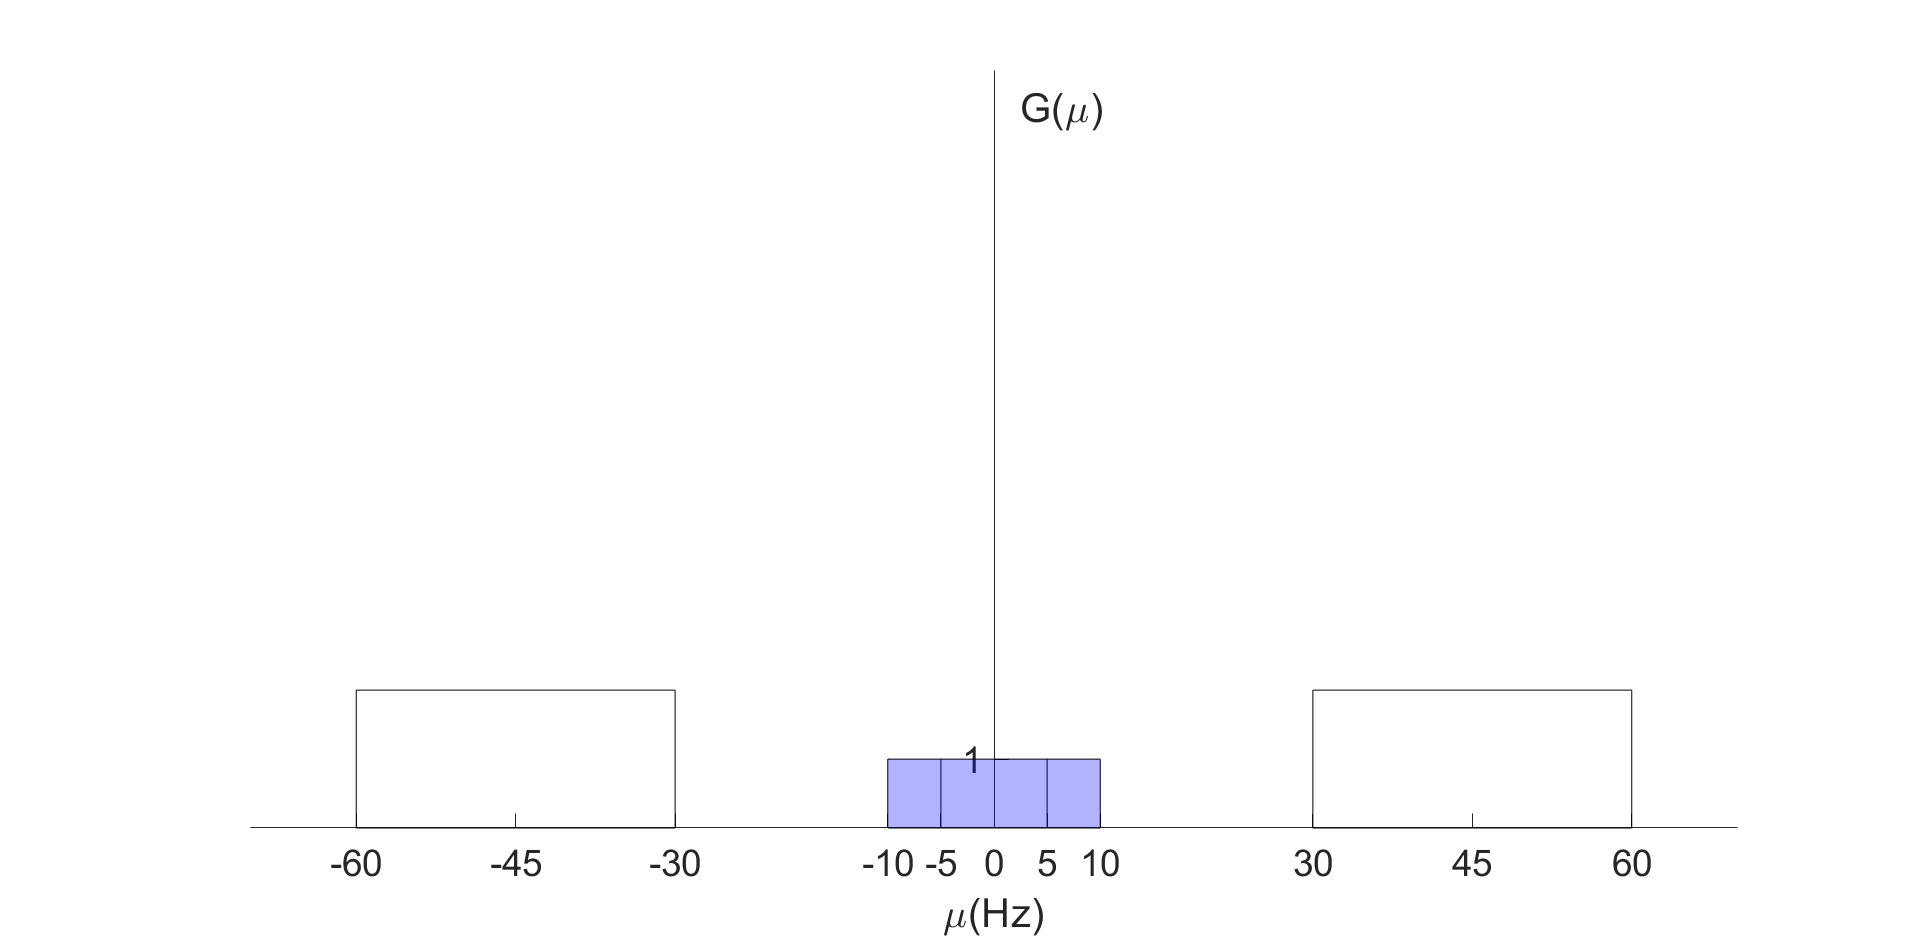
\includegraphics[width=\textwidth]{img/segnale_G.PNG}
		\caption*{Segnale $G\left(\mu\right)$.}
	\end{figure}
	
	\begin{figure}[!htp]
		\centering
		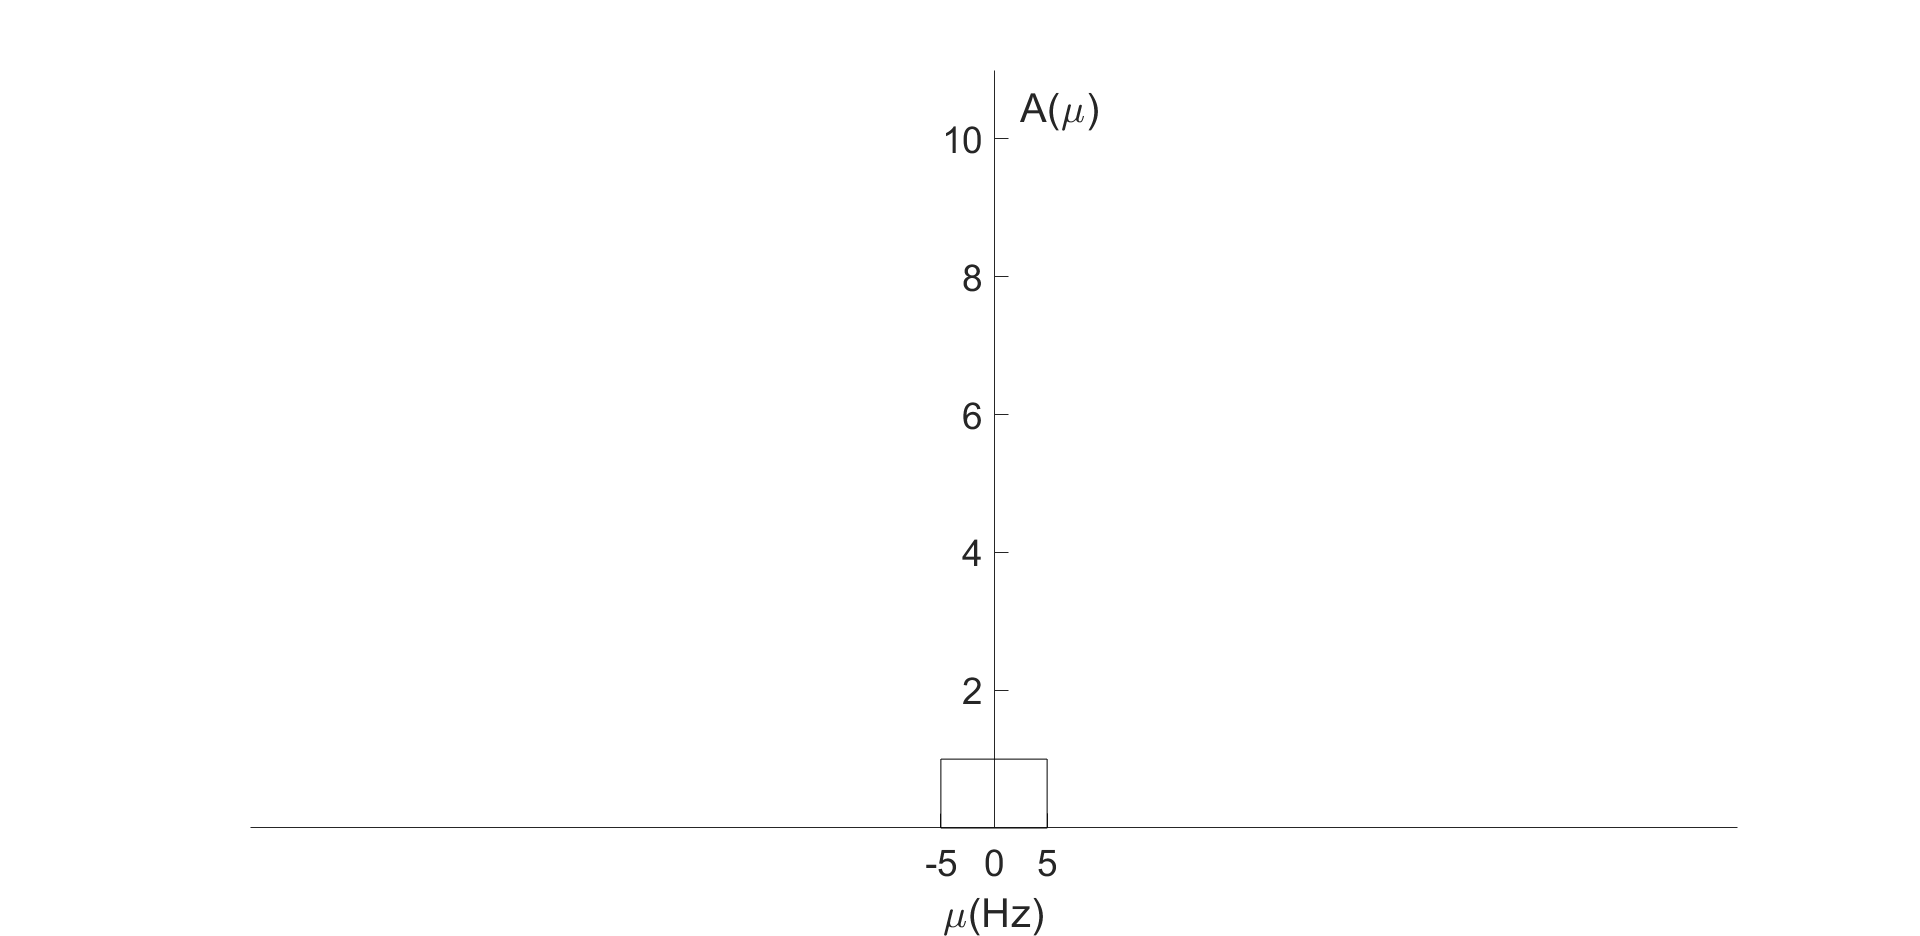
\includegraphics[width=\textwidth]{img/segnale_A.PNG}
		\caption*{Segnale $A\left(\mu\right)$ risultante.}
	\end{figure}
	
	\begin{figure}[!htp]
		\centering
		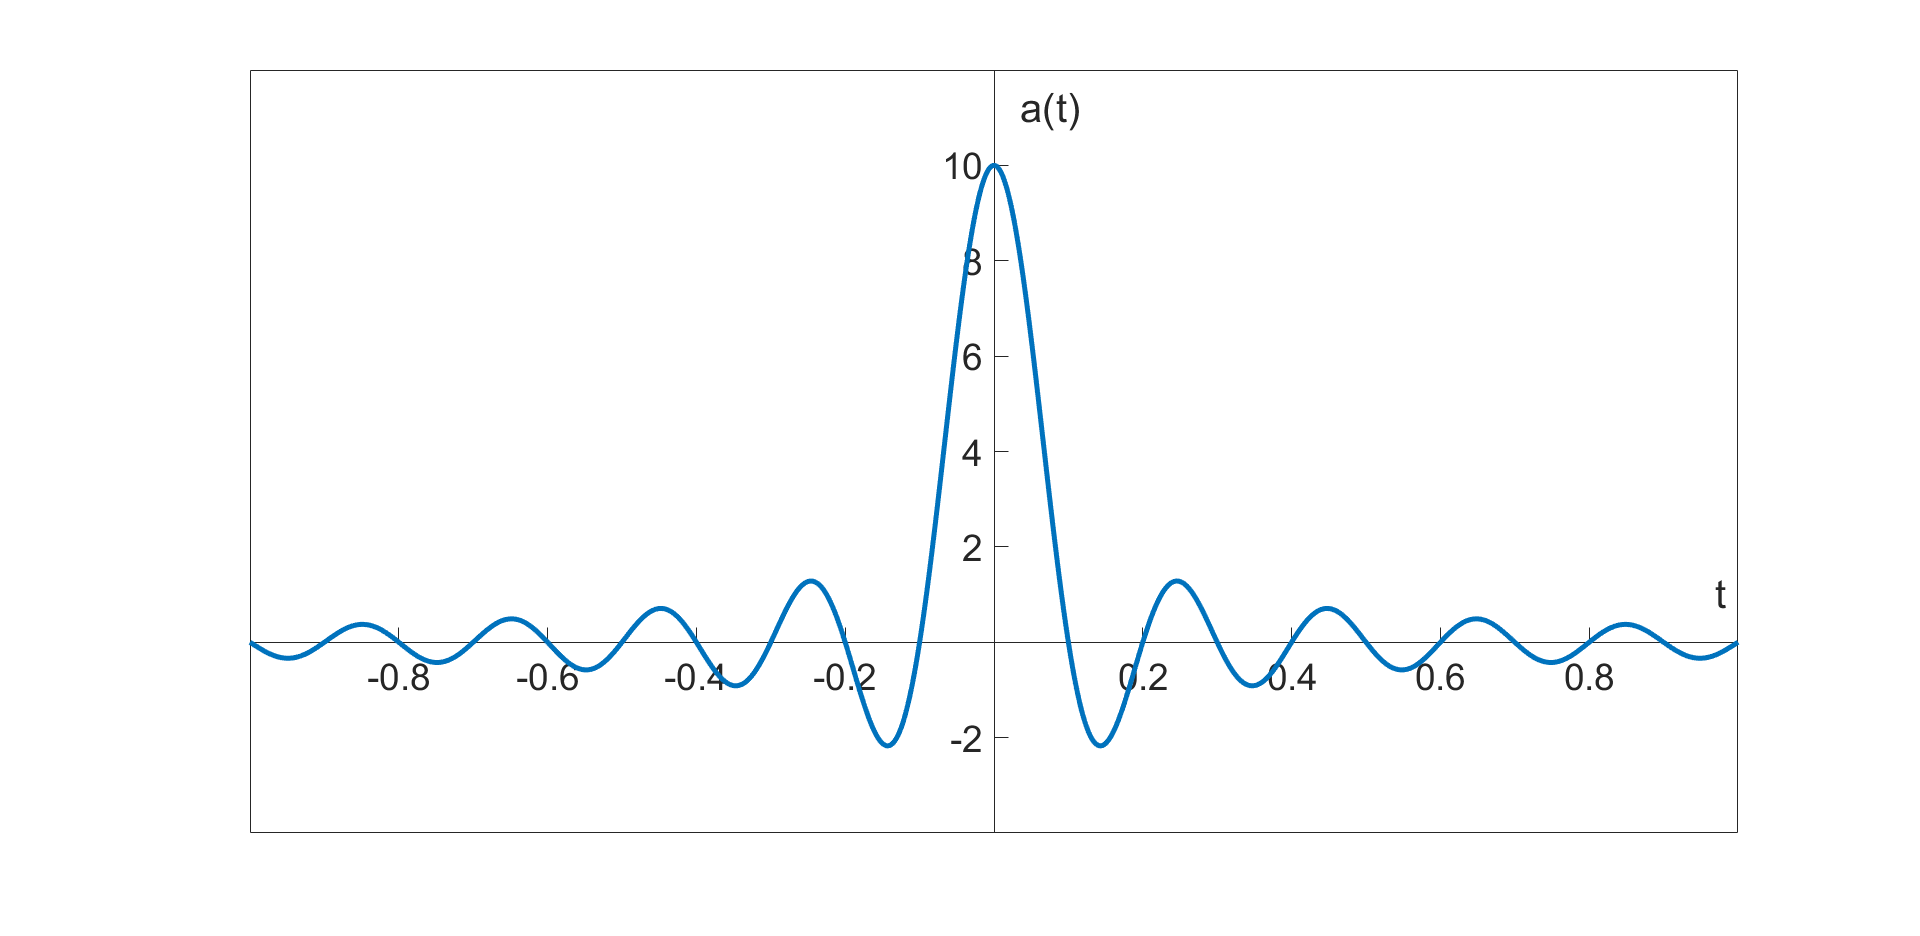
\includegraphics[width=\textwidth]{img/segnale_a-tempo.PNG}
		\caption*{Segnale nel dominio del tempo $a\left(t\right)$.}
	\end{figure}\newpage
	
	\noindent
	Adesso si esegue il \textbf{campionatore} a $10$ Hz. Attenzione: matematicamente parlando, campionare un segnale nel tempo significa moltiplicarlo per un treno di impulsi:
	\begin{equation*}
		\begin{array}{lllcl}
			\text{Dominio del tempo } & \longrightarrow & b\left(t\right) & = & a\left(t\right) \cdot \displaystyle\sum_{n = -\infty}^{\infty} \delta\left(t - \dfrac{n}{10}\right) \\
			&&&& \\
			\text{Dominio delle frequenze } & \longrightarrow & B\left(\mu\right) & = & A\left(\mu\right) * 10 \displaystyle\sum_{n = -\infty}^{\infty} \delta\left(\mu - 10n\right) \\
			&&& | & \\
			&&&=& \displaystyle\int_{-\infty}^{\infty} A\left(\tau\right) \cdot 10\displaystyle\sum_{n=-\infty}^{\infty} \delta\left(\mu - 10n - \tau\right) \mathrm{d}\tau \\
			&&&& \\
			&&& \downarrow & \text{Proprietà di setacciamento} \\
			&&&& \\
			&&&=& 10\displaystyle\sum_{n=-\infty}^{\infty} A\left(\mu - 10n\right) \\
			&&& | & \\
			&&&=& 10\displaystyle\sum_{n=-\infty}^{\infty} G\left(\mu - 10n\right) \cdot \Pi\left(\dfrac{\mu - 10n}{20}\right) \\
		\end{array}
	\end{equation*}
	\begin{figure}[!htp]
		\centering
		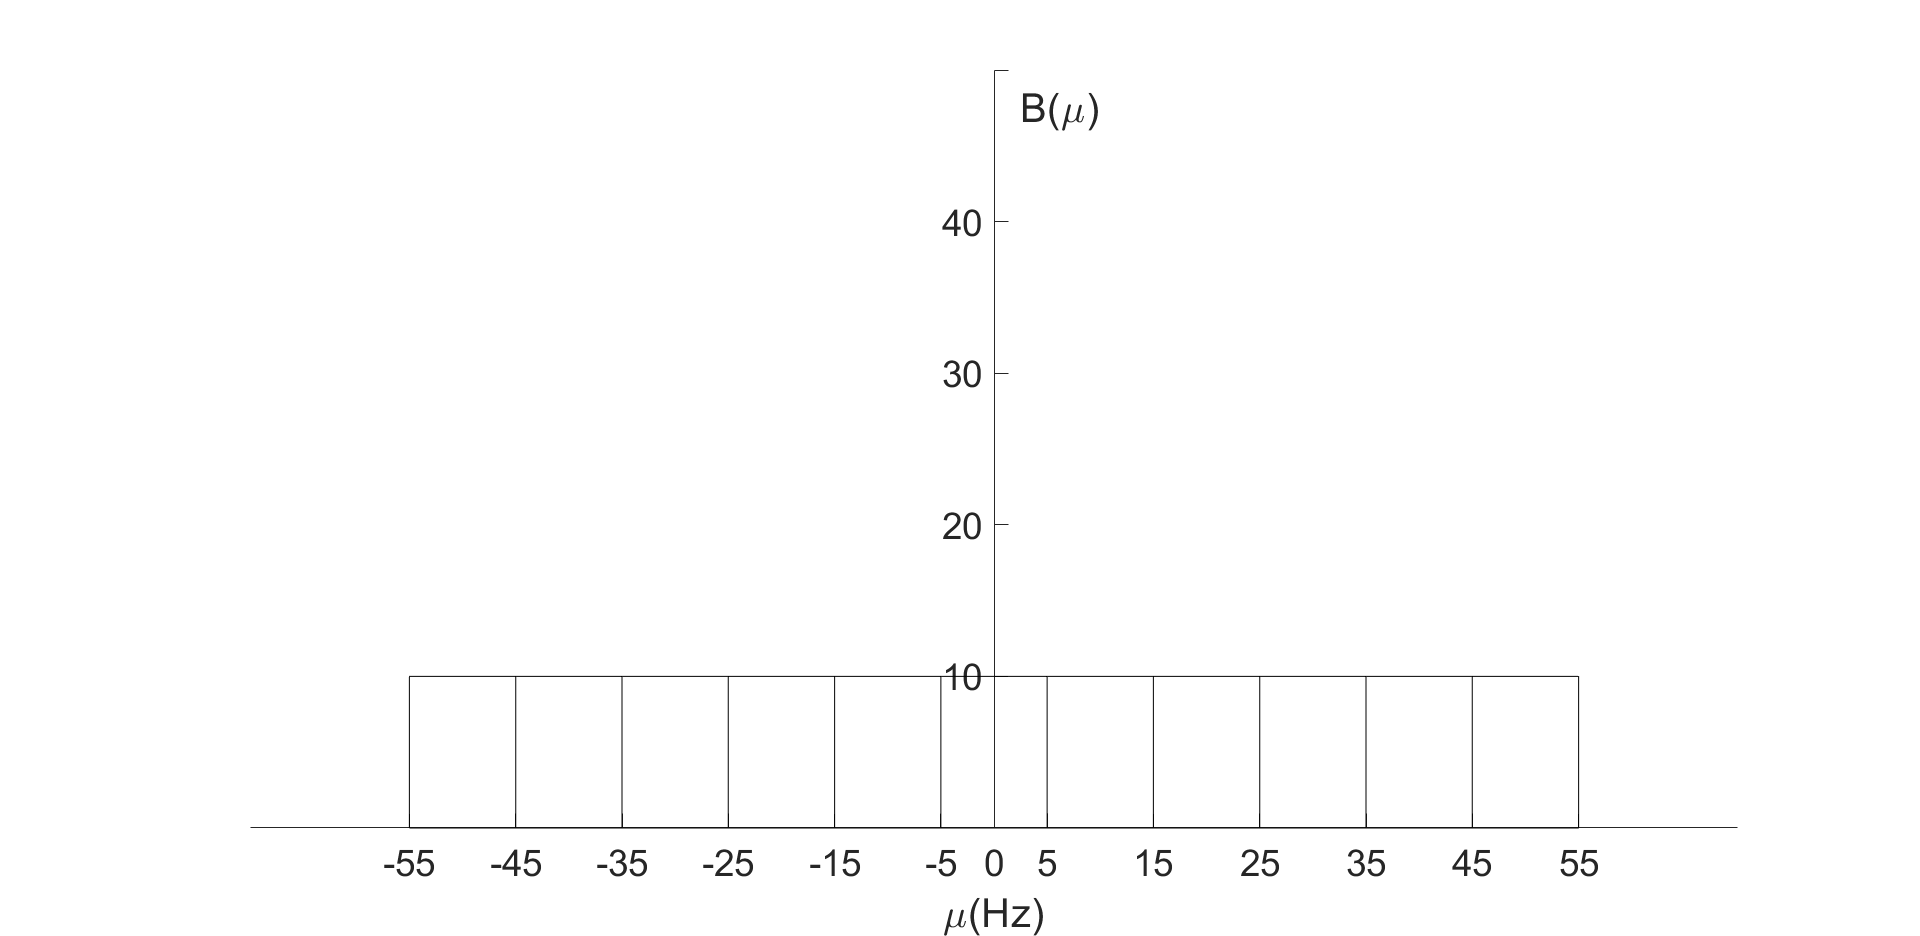
\includegraphics[width=\textwidth]{img/segnale_A-campionatore.PNG}
		\caption*{Il segnale $A\left(\mu\right)$ viene ripetuto ogni $10$ Hz.\newline
			\textbf{\underline{Attenzione}}: non c'è aliasing poiché non c'è sovrapposizione ma appaiamento.}
	\end{figure}\newpage
	
	\begin{figure}[!htp]
		\centering
		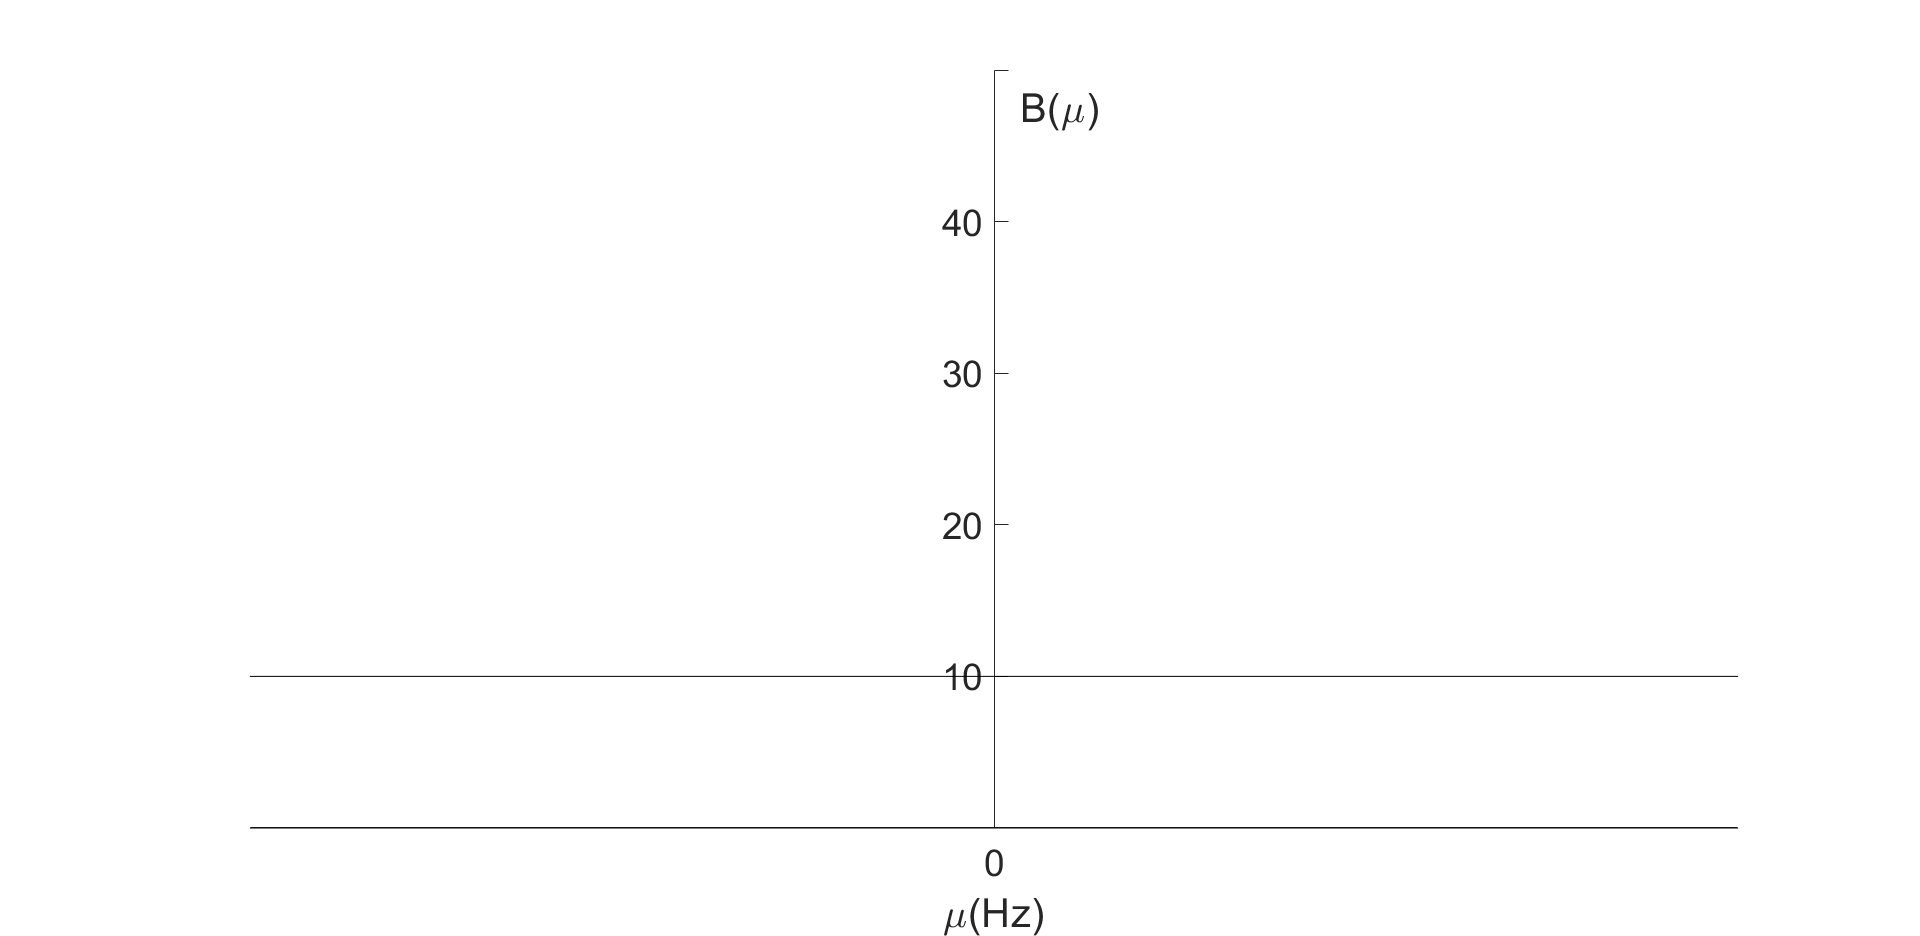
\includegraphics[width=\textwidth]{img/segnale_B.PNG}
		\caption*{Il segnale $B\left(\mu\right)$ risultante è costante a $10$.}
	\end{figure}
	
	\begin{figure}[!htp]
		\centering
		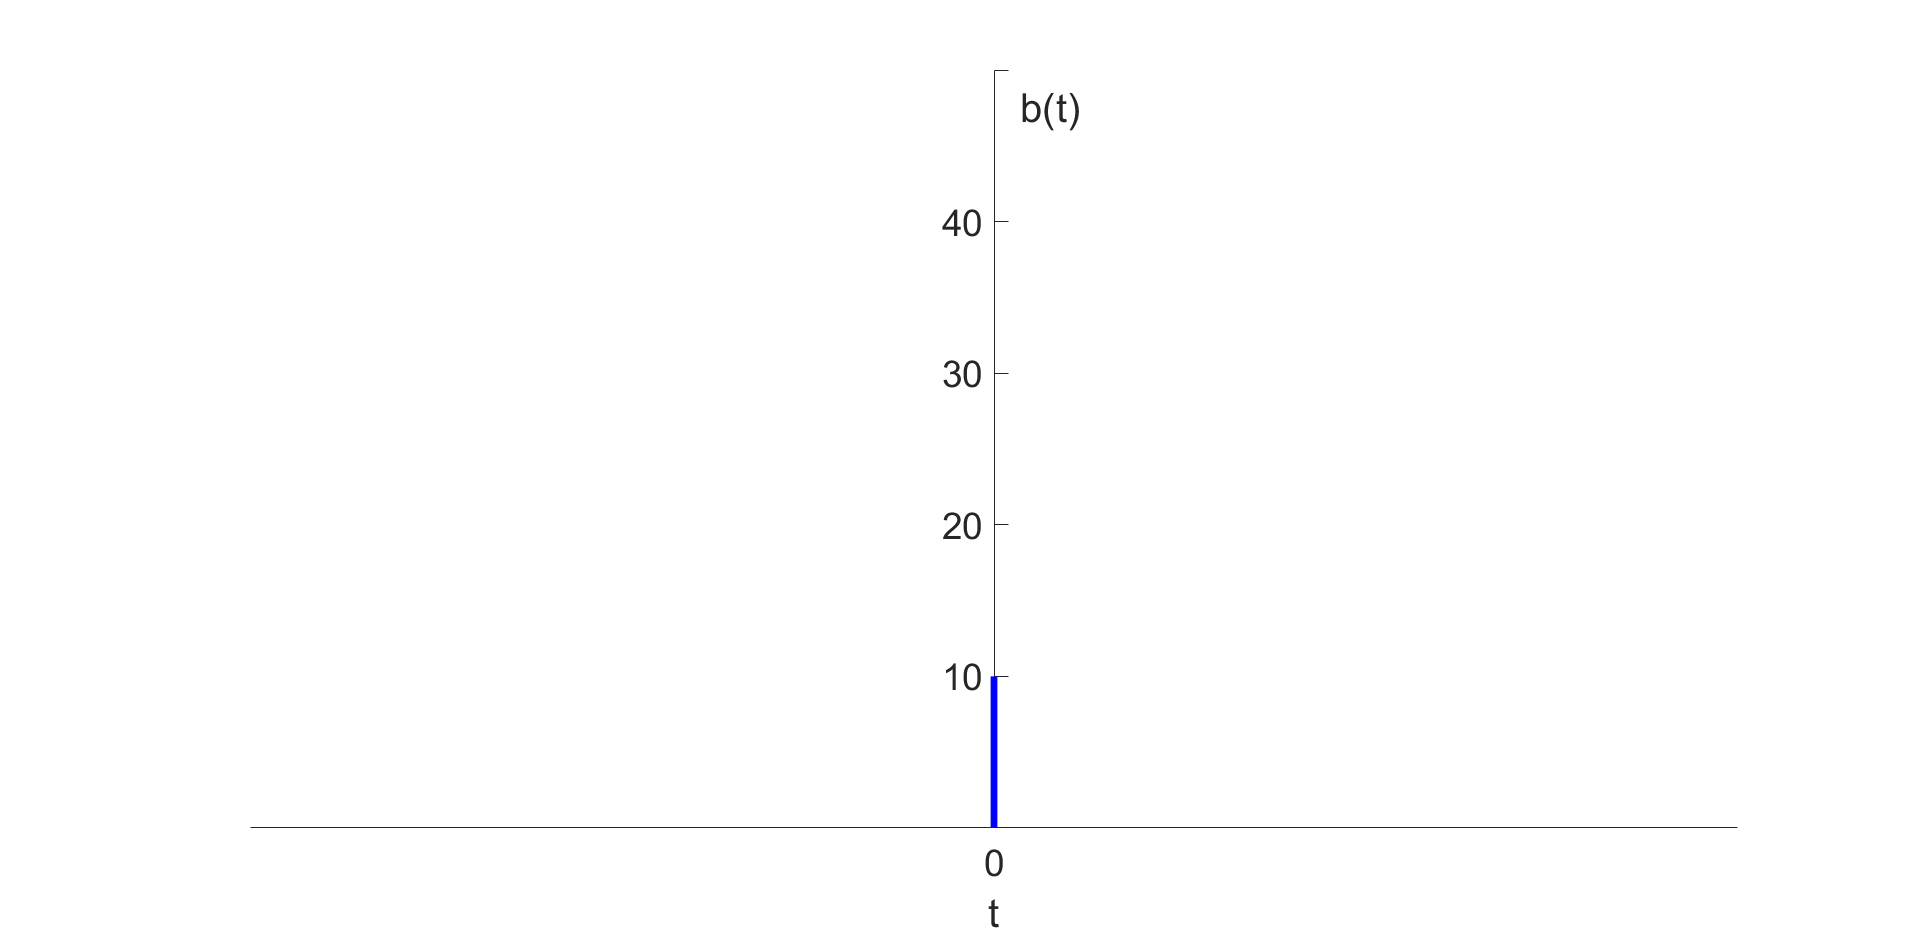
\includegraphics[width=\textwidth]{img/segnale_b-tempo.PNG}
		\caption*{Segnale nel dominio del tempo $b\left(t\right)$.}
	\end{figure}\newpage
	
	\noindent
	Infine, si applica l'ultimo filtro \textbf{passa basso ideale} con frequenza di taglio $25$~Hz:
	\begin{equation*}
		\begin{array}{lll}
			\text{Dominio del tempo } & \longrightarrow & c\left(t\right) = b\left(t\right) * 50\mathrm{sinc}\left(50t\right) \\
			&& \\
			\text{Dominio delle frequenze } & \longrightarrow & C\left(\mu\right) = B\left(\mu\right) \cdot \Pi\left(\dfrac{\mu}{50}\right)
		\end{array}
	\end{equation*}
	
	\begin{figure}[!htp]
		\centering
		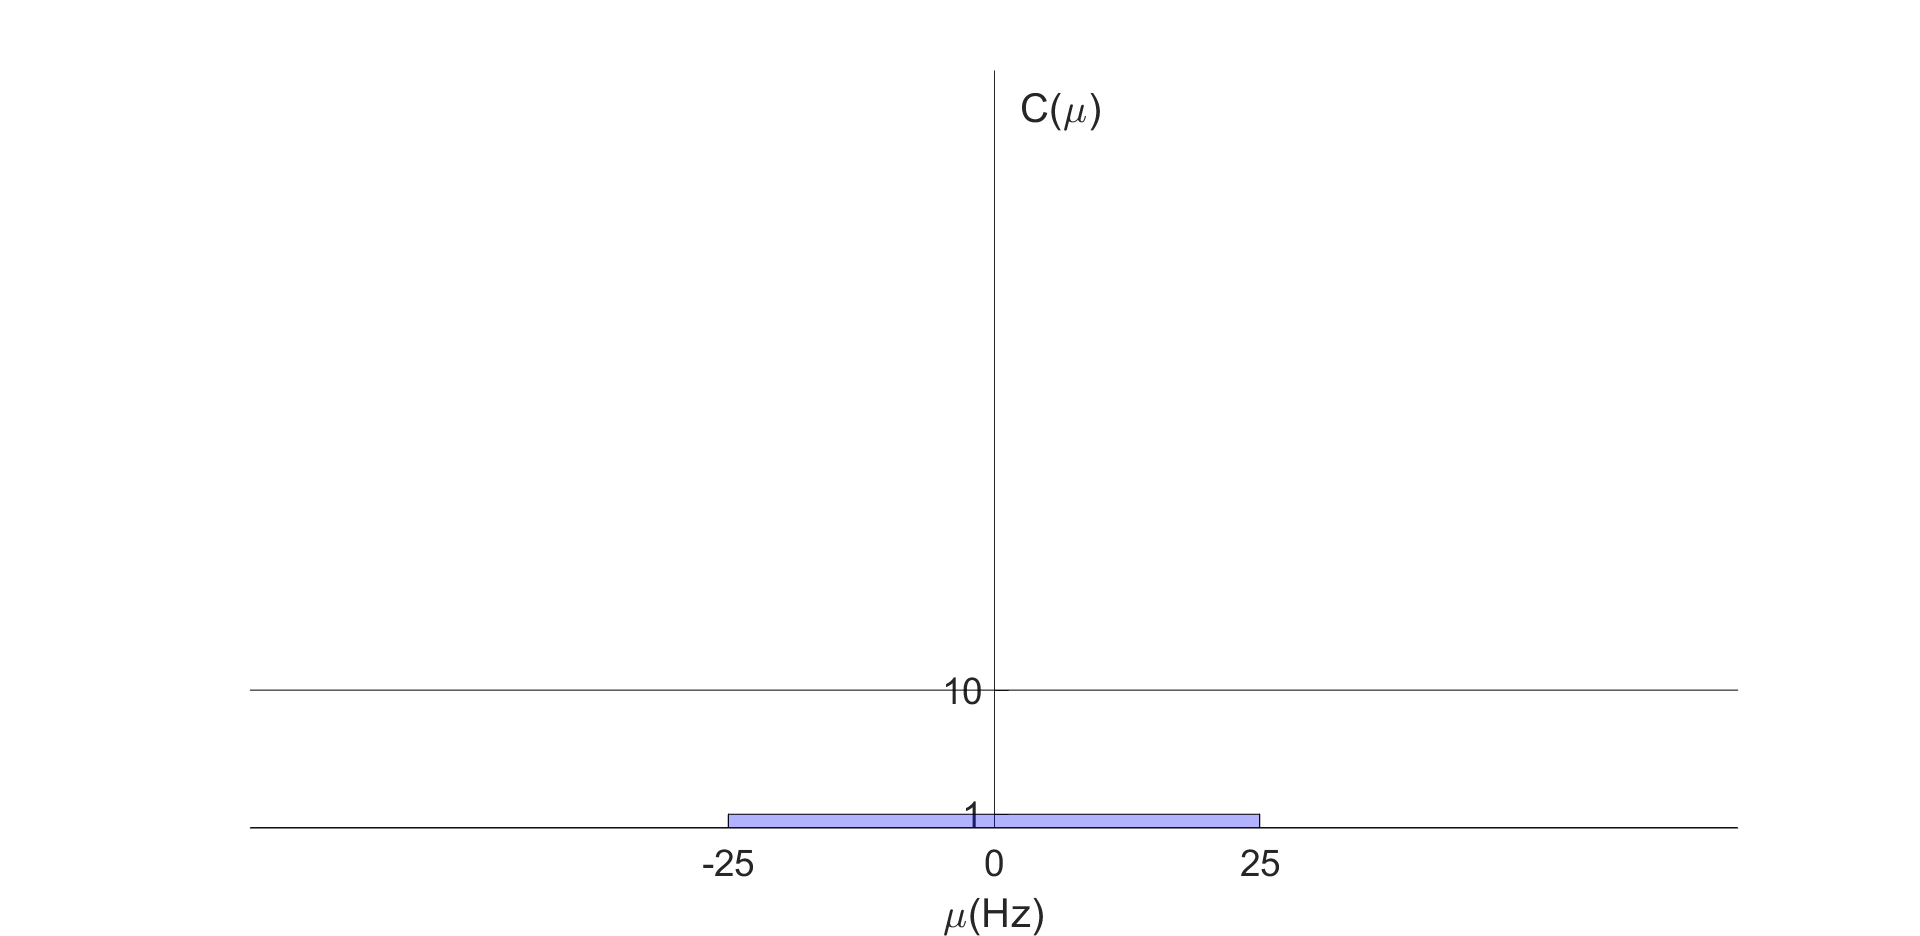
\includegraphics[width=\textwidth]{img/segnale_B-con-filtro.PNG}
		\caption*{Segnale $B\left(\mu\right)$ con il filtro passa basso ideale.}
	\end{figure}
	
	\begin{figure}[!htp]
		\centering
		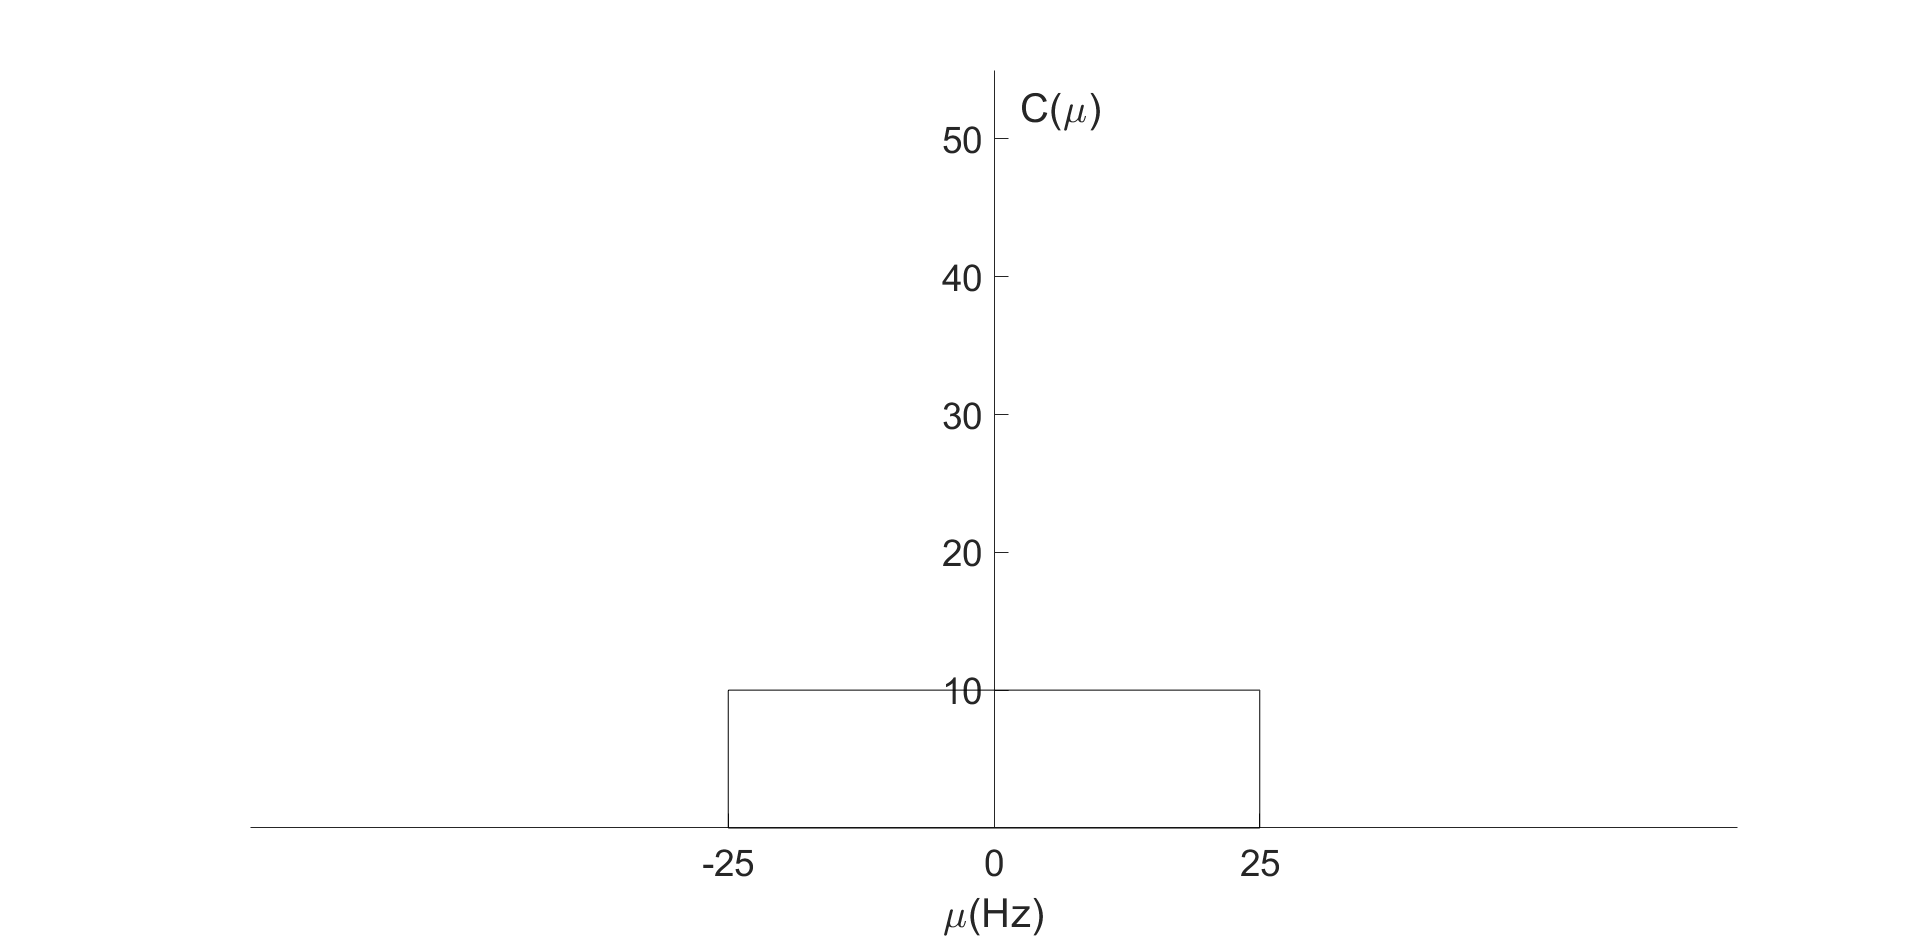
\includegraphics[width=\textwidth]{img/segnale_C.PNG}
		\caption*{Segnale $C\left(\mu\right)$ risultante.}
	\end{figure}\newpage
	
	\begin{figure}[!htp]
		\centering
		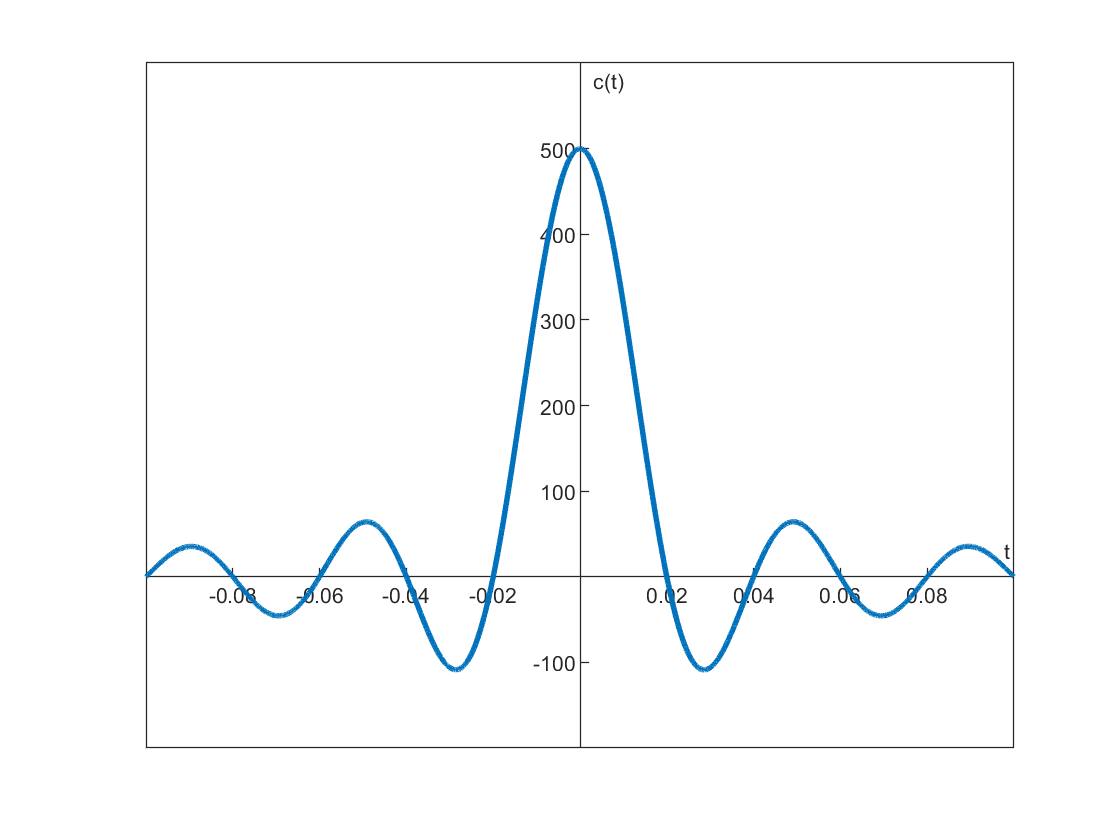
\includegraphics[width=\textwidth]{img/segnale_c-tempo.PNG}
		\caption*{Segnale nel dominio del tempo $c\left(t\right)$.}
	\end{figure}\newpage
	
	\section{Soluzione Esercizio}
	
	Le risposte alle domande:
	\begin{enumerate}
		\item 
		
		\item 
		
		\item 
	\end{enumerate}
\end{document}